\section{Einführung}

In unserer modernen, schnelllebigen Welt ist Stress zu einer allgegenwärtigen Erscheinung geworden. 
Angesichts der wachsenden Anforderungen im beruflichen und privaten Leben, einem Rückgang des Wirtschaftswachstums 
in der westlichen Welt und angespannten geopolitischen Verhältnissen erleben viele Menschen regelmäßig hohe Stresslevel, 
die zunehmend mit langfristigen gesundheitlichen Problemen, insbesondere Depressionen, in Verbindung gebracht werden \cite{Wang2008} \cite{Wang2001}.

Die Bürde psychischer Störungen war bereits vor der Covid-19-Pandemie ein prägendes Thema in der Gesellschaft, 
doch durch die Pandemie nahm das Ausmaß dieser Probleme noch weiter zu. Die Auswirkungen der globalen COVID-19-Pandemie 
haben weltweit zu einer signifikanten Zunahme von Depressionen und Angststörungen geführt. Laut einer Studie wurden 
während der Pandemie erhebliche Einflüsse von täglichen SARS-CoV-2-Infektionsraten auf die Prävalenz von schweren depressiven 
Störungen und Angststörungen beobachtet. Global gesehen stieg die Anzahl der Fälle von schweren depressiven Störungen um 
zusätzliche 53,2 Millionen (eine Zunahme von 27,6\%), was einer Gesamtprävalenz von 3152,9 Fällen pro 100.000 Einwohner entspricht, 
und die Fälle von Angststörungen stiegen um 76,2 Millionen (eine Zunahme von 25,6\%), was einer Gesamtprävalenz von 4802,4 Fällen 
pro 100.000 Einwohner entspricht \cite{Santomauro2021}.

In dieser Zeit wachsender Herausforderungen für die psychische Gesundheit sind innovative Ansätze zur Überwachung und Früherkennung 
von Stresssymptomen gefragter denn je. Die grundlegenden Arbeiten von Wissenschaftlern wie Walter B. Cannon und Hans Selye haben gezeigt, 
dass Stress nicht nur durch subjektive Erfahrungen gekennzeichnet ist, sondern sich auch durch messbare physiologische Veränderungen auszeichnet. 
Cannon beschrieb die „fight-or-flight“-Reaktion, während Selye die Stressreaktion und das General Adaptation Syndrome entwickelte, 
die erklären, wie Stress die körperliche Gesundheit beeinflusst \cite{Cannon1915} \cite{Selye1936}.

Prognosen zufolge sollen im Jahr 2028 allein über sechshundert Millionen Wearables, wie Smartwatches und Fitness-Tracker, 
ausgeliefert werden \cite{IDC2023}. Diese Geräte sind bereits heute in der Lage, entscheidende physiologische Marker wie Herzfrequenz, 
Schlafmuster und Aktivitätslevel zu erfassen, die Schlüsselindikatoren für die Erkennung von Stress sind. Trotz der Fähigkeit, 
wichtige physiologische Daten zu sammeln, konzentriert sich die Forschung bisher hauptsächlich auf klinische Sensoren. Die alltäglichen Wearables, 
die einen kontinuierlichen Zugang zu physiologischen Daten bieten, sind jedoch in der breiten Bevölkerung bereits weit verbreitet und könnten eine 
Schlüsselrolle bei der Früherkennung und dem Management von Stress spielen.

In dieser Arbeit wird untersucht, ob alltägliche Wearables im Verbund mit Algorithmen des maschinellen Lernens ein aussreichend akkurate Möglichkeit darstellen, um anhand durch Sensorik 
gemessener, physiologischer Marker, um Stresszustände in Echtzeit zu klassifizieren. Dazu wird zuerst ein Überblick über die diversen Definitionen von Stress und dessen Auswirkung auf physiologische Kenngrößen sowie 
die derzeit in alltäglichen Wearables verbaute Sensorik geschaffen. Danach wird ein kurzer empirischer Abschnitt aufgebaut, um die Valididtät der \ac{HRV} als Stressmarker zu unterstreichen.
Weiterhin werden Ansätze des maschinellen Lernens untersucht um zum Schluss eine Empfehlung über weitere Forschungsansätze zu geben.

\section{Theoretischer Rahmen Stress}
"The most significant feature of these bodily reactions in pain and in the presence of emotion provoking objects is that they are of the nature of reflexes" \cite{Cannon1915}. 
Diese Erkenntnis bildet das Fundament von Walter B. Cannons Forschungen, die zeigen, dass der Körper in als stressvoll wahrgenommenen Situationen, wie bei Schmerz und Hunger, 
Adrenalin ausschüttet. Cannon prägte den Begriff der "Homöostase", der den Prozess beschreibt, durch den der Körper ein inneres Gleichgewicht trotz externer Störungen aufrechterhält. 
Seine Arbeiten legen den Schwerpunkt auf die physiologischen Reflexe, bekannt als die "Fight-or-Flight"-Reaktion, die eine zentrale Rolle in der Aufrechterhaltung dieser Homöostase spielen.

Hans Selye, der in den 1930er Jahren den Begriff "Stress" wissenschaftlich prägte, erweiterte dieses Konzept durch die Einführung des General Adaptation Syndrome (GAS). Er definierte Stress als eine unspezifische Antwort des 
Körpers auf jegliche Art von Reizen, ob positiv oder negativ. Das GAS beschreibt, wie der Körper in drei Phasen auf Stressoren reagiert:

Alarmreaktion: Der Körper reagiert sofort auf einen Stressor, indem er Adrenalin freisetzt und den von Cannon beschriebenen "Fight-or-Flight"-Reflex auslöst, um die 
Homöostase schnell wiederherzustellen.
Resistenz-Phase: Bei anhaltendem Stress versucht der Körper, sich anzupassen und die Homöostase durch Regulation physiologischer und psychologischer 
Systeme aufrechtzuerhalten.
Erschöpfungs-Phase: Gelingt es dem Körper nicht, sich anzupassen, führt dies zu einer Erschöpfung, die gesundheitliche Schäden bis hin zum Tod zur Folge 
haben kann \cite{Selye1936}.

\subsection{Moderne Interpretation}

Aufbauend auf diesen grundlegenden Konzepten entwickelt sich die Definition von Stress aber durchaus mit wachsendem Forschungsstand weiter. 
In neueren Konzepten, wie von David S. Goldstein und anderen Wissenschaftlern entwickelt, wird Stress als eine bewusste oder unbewusste Bedrohung der 
Homöostase angesehen. Dieser Ansatz erkennt an, dass die Reaktion des Körpers auf Stress durchaus spezifisch sein kann, je nachdem, welche Herausforderung 
der Homöostase vorliegt, wie das Individuum den Stressor wahrnimmt und wie gut es sich in der Lage sieht, mit ihm umzugehen.

Goldstein hebt hervor, dass neben Cannons "sympathoadrenerges System", welches sich Allgemein auf das Zusammenspiel des Sympatischen Nervensystems 
und der Nebenniere zur wiederherstellung der Homöostase durch hormonelle Regulierung bezieht, zur Aufrechterhaltung der Homöostase auch das \ac{HPA-Achse}
eine zentrale Rolle in der Stressreaktion spielt. Beide Systeme sind aktiv an der Regulation und Anpassung bei Stress beteiligt und tragen dazu bei, eine 
neue Stabilität zu erreichen, die als "Allostase" bezeichnet wird.

Goldstein benutzt eine Analogie zu einem Heizkreislauf, um Allostase zu erklären: Ein Mensch stellt in einem Thermostat 
eine Soll-Temperatur ein; dieses Thermostat erfasst die aktuelle Raumtemperatur und aktiviert die Heizung, wenn die Temperatur unter den Sollwert fällt. 
Ähnlich reguliert der Körper durch Allostase die "innere Temperatur" oder physiologische Sollwerte, indem er nach Bedarf Anpassungen vornimmt, 
um Stabilität durch Veränderung zu erreichen.

Allostase beschreibt die Fähigkeit, Stabilität durch Veränderung zu erhalten, wobei "allostatische Last" die Kosten dieser Anpassungen misst. 
Diese Last kann, besonders bei langfristigem oder intensivem Stress, zu negativen gesundheitlichen Auswirkungen führen. Goldstein führt aus, 
dass zum Beispiel eine chronische Erhöhung des Blutdrucks, die zunächst dazu dient, die Durchblutung des Gehirns sicherzustellen, langfristig zu 
Gefäßschädigungen und daraus resultierenden Krankheiten wie Schlaganfall oder Herzinfarkt führen kann. \cite{Gold2007}

Das moderne Verständnis von Stress betont somit nicht nur die Akutreaktion des Körpers, sondern auch die langfristigen Auswirkungen der Stressbewältigung 
und die Bedeutung der Anpassungsmechanismen, die über die unmittelbare "Fight-or-Flight"-Reaktion hinausgehen.

\subsection{Physiologische Marker für Stress}

Wie bereits erleuchtet wurde, versucht der Körper verallgemeinert über zwei Systeme mit Stress umzugehen; der \ac{HPA-Achse} und dem sympathoadrenergem System. 
Das sympathoadrenerge System bewirkt eine Auscchüttung von Adrenalin sowie Noradrenalien, welche in kurzer Zeit physiologische Anpassung wie einer Erhöhung des Blutdrucks bewirken,
wohingegen die \ac{HPA-Achse} etwas langsamer über Anregung von Cortisolproduktion fungiert. \cite{Kaiser2023}

Da sich diese Arbeit darauf fokusiert, Stress anhand messbarer physiologischer Merkmale zu klassifizieren, widmen wir einen etwas ausführlicheren Blick auf folgendes Paper von Ernst:

Die Studie umfasst einen multimodalen Ansatz um pyhsiologische Marker in akuten Stresssituationen aufzuzeichnen und auszuwerten. In fünfundsechzig gesunden Teilnahmern wurden mithilfe des 
\ac{MMST}, einen verschiedenen Komponenten umfassenden Test, darunter kognitive Aufgaben und sensorische Stimulation, eine kontrollierte, akute Stressreaktion erzeugt. Während des Test wurden mit 
Hilfe einer Kombination von Biosensorik wie \ac{EKG} und \ac{PPG} und Selbstevaluierungsbögen sechzig verschiedene physiologische Marker aufgezeichnet, darunter Herzratenvariablilität, Hautleitfähigkeit, Atmungsrate und mehr.
Weiterhin wurden über unter anderem Speichelproben die Konzentrationen von Cortisol gemessen, um eine Aktivierung der \ac{HPA-Achse} nachweisen zu können. 

Diese wurden einer statistischen Untersuchung unterzogen, um die Differenzen zwischen diesem Markern im Ruhezustand im Vergleich zum Stresszustand aufzuzeigen. Demzufolge wurde unter anderem eine Reduktion der Herzratenvariablilität; 
herausgerechnet als \ac{RMSSD} aus den \ac{EKG} Messungen, von im Schnitt 46.0 ± 18.2 Millisekunden auf 37.3 ± 16.1 Millisekunden, was einer Differnenz des Durschnittes 
von 19 Prozent bedeutet, festgestellt. \cite{Ernst2023}

Insgesamt deckten sich die Ergebnisse weitgehend mit Erkenntnissen anderer Literatur sowie mit den Standartisierten Selbstevaluierungsbögen, womit ein wissenschaftlich zuverlässiger Rahmen an bedeutenten physiologischen Markern
zur Erkennung von Stress geschaffen wurde, an dem wir uns in dieser Arbeit noch weitergehend bedienen werden.


\section{Wearables}

Wie eingangs bereits erwähnt ist der Markt für Wearables gigantisch und soll im Jahr 2028 eine Auslieferungszahl von sechshundert Millionen Stück erreichen. Insbesondere Smartwatches und 
Fitnesstracker erfreuen sich in Europa einer steigenden Popularität, wonach laut einer Statista Umfrage in Deutschland im Jahre 2023 bereits fünfunddreisig Prozent ein solches nutzen (Vergleich 2021: neunzehn Prozent). \cite{bocksch2023nutzung}

Insbesondere diese eröffnen breite Möglichkeiten zur Erfassung von Stress, da viele dieser Wearables nicht invasive Biosensorik verbaut haben, und sowieso schon alltäglich getragen werden. Um eingrenzend tiefer auf die technologischen Merkmale eingehen 
zu können, fokussieren wir uns auf die Apple Watch, welche nach geschätzen Absatzzahlen aus dem Jahr 2020 mit über 33 Millionen Stück eine große Marktdominanz zeigte. \cite{bocksch2021apple}



\subsection{Technologische Grundlagen Wearables}

Es wird kurz die für die Erfassung von physiologischen Stressmarker wichtigste Sensorik der Apple Watch beleuchtet. Dabei werden speziell auf die \ac{PPG} und das \ac{EKG} eingegangen, da diese genutzt werden um die obig erwähnte wichtige \ac{HRV} zu berechnen.

\subsubsection{Photoplethysmographie}
\ac{PPG} ist eine kostengünstige Methode um zahlreiche Marker des Herz-Kreislaufes zu erfassen, indem ein Lichtsignal, meist im Infrarot-Beriech, entsendet wird und mittels Photodioden gemessen wird, 
wie viel dieses Lichts vom mikrovaskulären Blut absorbiert wurde. Da sich das Blutvolumen im Laufe des Herzschlagszyklus ändert, 
kann bei wiederholten Messung die Herzfrequenz sowie andere daraus resultierende Werte errechnet werden. \cite{Allen2007}. 

Ein solcher Sensor ist in jeder Apple Watch verbaut, welche Stand jetzt auf den Markt kam. Die Apple Watch benutzt Grüne-LEDs, welches mehrer hundert male pro Sekunde leuchten, wobei das reflektierte Licht 
von Photodioden gemessen wird. Weiterhin besitzt der \ac{PPG} Sensor der Apple Watch einen Hintergrundoperationsmodus, welcher für durchgängige Messungen im Hintergrund mit Infrarot fungiert.

Tatsächlich benutzt jede Apple Watch die \ac{PPG} Messungen zur Ermittlung der \ac{HRV}, sowie zur Erfassung der Herzfrequenz und der Blutsauerstoffsättigung.\cite{Apple2023}

\subsubsection{Elektrokardiogramm}

Das Herz fungiert auf der Basis von rhytmischen An- und Entspannen der Vorhöfe und Herzkammern. Dieser Vorgang wird durch elektrische Potentiale angestossen, welche mit Hilfe eines \ac{EKG}s gemessen werden können.

Seit der Einführung der Apple Watch Series 4 ist ein \ac{EKG} Bestandteil der Sensorausstattung. Dieses erfasst die elektrischen Signale der Herzmuskeln durch spezielle Sensoren an der Rückseite der Uhr und der digitalen Krone, welche der Nutzer mit der nicht dominanten Hand für circa 30 Sekunden berühren muss und so den Stromkreis schließt. 


\subsubsection{Weiter relevante Sensorik}

Die Apple Watch verfügt noch über weiter Sensorik, welche zur Klassifizierung von Stress nütliche Daten liefern kann. Ein Mikrofon kann benutz werden um Änderungen an der Stimmlage festzustellen, wohingegen das verbaute 3-Achsen Gyroskop und der Beschleunigungssensor benutz werden können um Körperbewegungen wahrzunehmen. Óscar Martínez Mozos et al. benutzen diese Metriken in Kombination mit \ac{EKG} und \ac{PPG} Daten klinischer Sensoren um mittels des Klassifizierungsalgorithmen \ac{SVM} und dem Metalgortihmus \ac{AdaBoost} binär zwischen nicht-Stress und Stress zu klassifiziern. \cite{Mozos2017StressDU} 

Auch wenn diese Sensorik keine Daten zu den physiologischen Markern ermittelt, auf welche sich in dieser Arbeit fokussiert wird, behalten wird diese für supplementäre Features im Hinterkopf.


\subsection{Limitationen von Wearables}

Eine Limitation der Apple Watch könnte die Messgenauigkeit der verbauten Sensorik sein. Hernando et al. validierten in einer Studie die Genauigkeit der aus den RR-Intervalle, welche die Apple Watch mithilfe der \ac{PPG} aufzeichnet, herausgerechneten Herzfrequenz sowie \ac{HRV}. Zwanzig Teilnehmer trugen ein Validierungsgerät und eine Apple Watch 4 während einer 5-minütigen Ruhephase und einer 5-minütigen Phase, in welcher mittels des Stroop Test leichter Stress induziert wurde. 

Die Studie ergab nach Synchronisation der Signale und statistischer Auswertung eine serhr gute Übereinstimmung jeweils in den rohen RR-Intervallen, als auch in der Herzfrequenz und der \ac{HRV}. Gleichzeitig wurde aber auch festgestellt, dass die Apple Watch vermehrt RR-Intervalle nicht identifizieren konnte, was der Autor auf eine Nichterkennung des \ac{PPG}-Pulses zurückführt, was bei nicht richtigem Sitz beziehungsweise vor allem auch viel Bewegung passieren kann. 

Dies beeinträchtigt die Messergebnis nicht erwähnenswert, gilt aber im Auge behalten zu werden, da verinzelt fehlende RR-Intervalle insbesondere die \ac{HRV}, welche beispielsweise aus der Standardabweichung der Abstände zwischen RR-Intervallen berechnet werden kann, beeinflussen. \cite{s18082619}

Ähnliche Erkenntnisse bereichten auch B. Bent et al., welche vier Konsumer-Wearables, Apple Watch 4 inkludiert, und zwei Wearables in Forschungsqualität gegen ein \ac{EKG} als Referenzstandard gebenchmarked haben. Dabei wurden dreiunffünfzig Teilnehmer in jeweils drei Runden, umfassend einer Ruhephase im Sitzen, tiefen Atmens, körperlicher Aktivät und einer folgenden Ruhephase, mit Geräten ausgestattet, um pro Teilnehmer eine Messung der Herzfrequenz jedes Wearables zu haben. 
Sie berichten von einer höheren Genauigkeit der Herzfrequenz der Konsumer-Wearables im Ruhezustand als die der Forschungsgeräte, bestätigen aber Hernandos et al. Vermutung, dass die Messungen bei körperlicher Aktivität niedrigere Qualität aufweisen. \cite{Bent2020}

Bei dieser Studie wurden die Teilnehmer auch extra nach diversen Hautfarbtönen ausgewählt, um zu untersuchen ob die Hautfarbe einen Einfluss auf die Qualität der Herzfrequenzmessung hat, was Aufgrund der Absorbtionsfähigkeit von Melanin eine oft vermutete Limitation von \ac{PPG}-Messungen ist. B. Brent et al. konnten keine Korrelation zwischen dem Hautfarbton und der Messungenauigkeit aufzeigen, was aber kritisch zu betrachten ist, da dies nur bedingt dem Konsens anderer Studien folgt.

Die Genauigkeit von alltäglichen Wearables scheint vielversprechend zu sein, es geilt zu beachten, dass dies während körperlicher asktivität abweichen kann und im Raum steht, dass \ac{PPG} einen Racial-Bias beinhält, welcher physisch bedingt ist, aber nichtsdestotrotz vorallem bei prediktiven medizinischen Verfahren so gut es geht eliminiert werden muss.

\section{Validierung Wesad Dataset}

Um die Erkenntnisse von H. Ernst et al. zu reproduzieren und im anbetracht der obig genannten Limitation, welche sich hauptsächlich auf \ac{PPG} beziehen, möchte ich einen eigenen kleinen empirischen Anteil anhand des WESAD-Datensatzes \cite{Schmidt2018WESAD} beitragen. Es wird versucht aus dem im Datensatz gegebenem \ac{EKG}-Signal die Änderung der Herzfrequenz sowie der Herzratenvariabliltät von der Baseline zum Stresszustand zu errechnen.

\subsection{Begebenheiten des Datensatzes}
Der Datensatz umfasst physiologische und Bewegungsdaten, die von 17 Teilnehmern (zwei Teilnehmer sind aufgrund von Komplikationen der Sensorik ausgeschieden) während einer Laborsitzung mit einem an der Brust und einem am Handgelenk getragenen Gerät aufgezeichnet wurden. Das an der Brust befestigte Gerät zeichnete ein 3-Elektroden \ac{EKG} mit einer Abtastrate von 700Hz auf, welches genauer untersucht wird.

Die Studie wurde mit einem definierten Protokoll durchgeführt, das darauf abzielte, verschiedene emotionale Zustände zu induzieren:

Baseline-Zustand: Die Teilnehmer ruhten sich aus, während sie neutrales Lesematerial zur Verfügung hatten.

Amusement-Zustand: Die Teilnehmer sahen sich eine Reihe von lustigen Videoclips an.

Stress-Zustand: Dies wurde durch den \ac{TSST} induziert, der öffentliches Sprechen und mentale Arithmetikaufgaben umfasste.

Meditationsperioden: Nach den Stress- und Amusement-Bedingungen führten die Teilnehmer eine geleitete Meditation durch, um sie zu beruhigen.

Ausserdem wurde die Studie multimodal ausgelegt, wobei die Teilnehmer nach dem Durchlauf des Protokolls mehrere Fragebögen zur Selbstevaluierung des Empfindes während des Protokolls
ausfüllten.

\subsection{Auswertung der EKG-Daten}

Der Datensatz enthält eine Python-Pickle pro Teilnehmer mit den sychronisierten Sensor-Daten sowie den jeweiligen Labels, wobei 0 die Baseline-Messungen und 2 die Stress-Messungen darstellt.
Es sind noch Labels für 'Amusement' und anderweitige Zustände verfügbar, diese wurden aber nicht berücksichtig.

Weiterhin beinhaltet jeder Teilnehmer-Orderner einer Textdatei, in welcher unter anderem angemerkt wurde, ob ein Teilnehmer beispielsweise vor der Studie raucht, Koffein konsumierte oder Sport bertrieb. Es werden sich nur Teilnehmer angeschaut, welche all diese Anmerkungen mit 'Nein' beantworteten.

Die Pickle Dateien wurde in ein Pandas DataFrame geladen. Darauf wurden pro Teilnehmer Teilsegmente von jeweils 30-Sekunden bestimmt, was bei einer Abtastrate von 700Hz genau 21.000 Datenpunkten entspricht. Segmente welche nicht die Anzahl dieser Datenpunkte erfüllen konnten (die letzten einer Messreihe eines Teilnehmers) wurden nicht beachtet. 
Das Label welches für ein Segment galt, wurde über ein Mehrheitsvotum der Label der einzelnen Datenpunkte bestimmt. 

Mithilfe des Packages neurokit2, welches speziell für \ac{EKG}-Signale parametriesierte Filter anwendet, wurden pro Segment die R-Peaks bestimmt aus welchen die RR-Intervalle berechnet wurde. Siehe Abbildung 1.

\begin{figure}[ht]
    \centering
    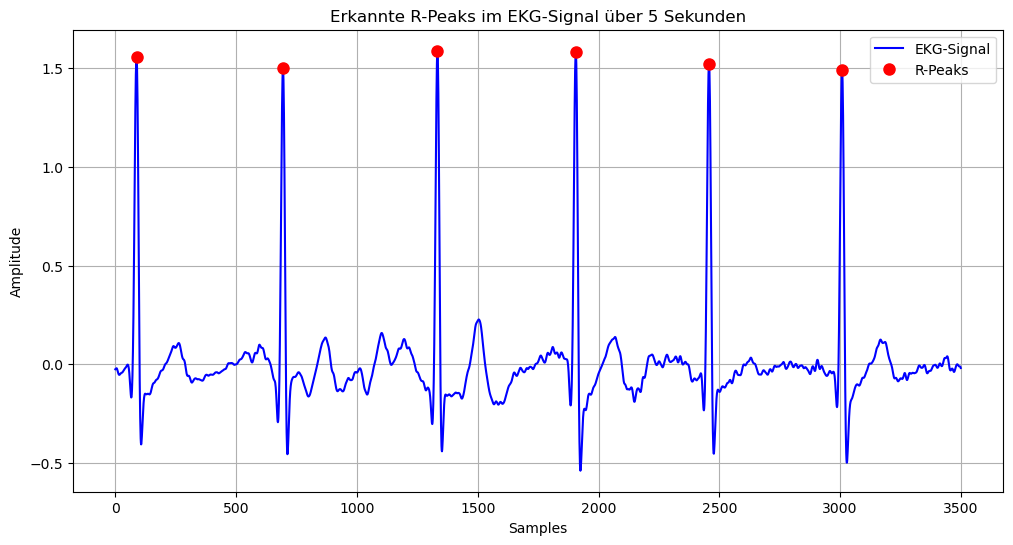
\includegraphics[width=1\textwidth]{Bilder/EKG-Plot.png}
    \caption{Erkannte R-Peaks im 12-Sekunden-Ausschnitt des gefilterten EKG-Signals}
    \label{fig:ekg-peaks}
\end{figure}

Mit diesen konnte pro Segment die Durchschnittliche Herfrequenz sowie die \ac{HRV} mittels \ac{RMSSD} wie folgt:

\[
\text{RMSSD} = \sqrt{\frac{1}{N-1} \sum_{i=1}^{N-1} (RR_i - RR_{i+1})^2}
\]

berechnet werden.

Daraufhin wurden alle Segmente entfernt, welche nach dem Majority-Voting nicht mit Baseline oder Stress gelabelt wurden.

\subsection{Bewertung und Diskussion}

Im Tabelle 1 werden die durschnittliche Herzfrequenz und \ac{HRV} pro Teilnehmer pro Label aufgezeigt, als auch die prozentuale Veränderung von Baseline zu Stress.

Über alle berücksichtigten Teilnehmer veränderte sich die Herzfrequenz um $\mathbf{28.874\% \pm 17.287}$ und die HRV\textsubscript{RMSSD} um $\mathbf{-46.676\% \pm 22.230}$.

\begin{table}[hp]
    \begin{tabular}{ccccccc}
    \rowcolor[HTML]{9B9B9B} 
    \multicolumn{1}{l}{\cellcolor[HTML]{9B9B9B}}                                      & \multicolumn{2}{c}{\cellcolor[HTML]{9B9B9B}\textbf{Kein Stress}}                                                               & \multicolumn{2}{c}{\cellcolor[HTML]{9B9B9B}\textbf{Stress}}                                                                   & \multicolumn{2}{c}{\cellcolor[HTML]{9B9B9B}\textbf{Delta}}                                                                     \\
    \rowcolor[HTML]{C0C0C0} 
    \multicolumn{1}{l}{\multirow{-2}{*}{\cellcolor[HTML]{9B9B9B}\textbf{Teilnehmer}}} & \begin{tabular}[c]{@{}c@{}}HR\_Mean \\   {[}BPM{]}\end{tabular} & \begin{tabular}[c]{@{}c@{}}HRV\_Mean\\ {[}ms{]}\end{tabular} & \begin{tabular}[c]{@{}c@{}}HR\_Mean \\ {[}BPM{]}\end{tabular} & \begin{tabular}[c]{@{}c@{}}HRV\_Mean \\ {[}ms{]}\end{tabular} & \begin{tabular}[c]{@{}c@{}}HR\_Delta \\ {[}\%{]}\end{tabular} & \begin{tabular}[c]{@{}c@{}}HRV\_Delta\\  {[}\%{]}\end{tabular} \\ \hline
    \multicolumn{1}{|c|}{S2}                                                          & \multicolumn{1}{c|}{72.99}                                      & \multicolumn{1}{c|}{96.38}                                   & \multicolumn{1}{c|}{76.91}                                    & \multicolumn{1}{c|}{43.07}                                    & \multicolumn{1}{c|}{5.36}                                     & \multicolumn{1}{c|}{-55.31}                                    \\ \hline
    \multicolumn{1}{|c|}{S3}                                                          & \multicolumn{1}{c|}{60.99}                                      & \multicolumn{1}{c|}{130.06}                                  & \multicolumn{1}{c|}{86.29}                                    & \multicolumn{1}{c|}{55.63}                                    & \multicolumn{1}{c|}{41.48}                                    & \multicolumn{1}{c|}{-57.23}                                    \\ \hline
    \multicolumn{1}{|c|}{S4}                                                          & \multicolumn{1}{c|}{64.75}                                      & \multicolumn{1}{c|}{80.48}                                   & \multicolumn{1}{c|}{79.62}                                    & \multicolumn{1}{c|}{42.05}                                    & \multicolumn{1}{c|}{22.96}                                    & \multicolumn{1}{c|}{-47.76}                                    \\ \hline
    \multicolumn{1}{|c|}{S10}                                                         & \multicolumn{1}{c|}{92.09}                                      & \multicolumn{1}{c|}{33.37}                                   & \multicolumn{1}{c|}{107.13}                                   & \multicolumn{1}{c|}{29.90}                                    & \multicolumn{1}{c|}{16.33}                                    & \multicolumn{1}{c|}{-10.40}                                    \\ \hline
    \multicolumn{1}{|c|}{S13}                                                         & \multicolumn{1}{c|}{84.92}                                      & \multicolumn{1}{c|}{35.80}                                   & \multicolumn{1}{c|}{108.32}                                   & \multicolumn{1}{c|}{19.30}                                    & \multicolumn{1}{c|}{27.56}                                    & \multicolumn{1}{c|}{-46.08}                                    \\ \hline
    \multicolumn{1}{|c|}{S14}                                                         & \multicolumn{1}{c|}{88.51}                                      & \multicolumn{1}{c|}{29.21}                                   & \multicolumn{1}{c|}{126.90}                                   & \multicolumn{1}{c|}{11.22}                                    & \multicolumn{1}{c|}{43.36}                                    & \multicolumn{1}{c|}{-61.58}                                    \\ \hline
    \multicolumn{1}{|c|}{S15}                                                         & \multicolumn{1}{c|}{80.01}                                      & \multicolumn{1}{c|}{46.45}                                   & \multicolumn{1}{c|}{84.94}                                    & \multicolumn{1}{c|}{42.33}                                    & \multicolumn{1}{c|}{6.16}                                     & \multicolumn{1}{c|}{-8.86}                                     \\ \hline
    \multicolumn{1}{|c|}{S16}                                                         & \multicolumn{1}{c|}{86.99}                                      & \multicolumn{1}{c|}{36.48}                                   & \multicolumn{1}{c|}{128.14}                                   & \multicolumn{1}{c|}{11.21}                                    & \multicolumn{1}{c|}{47.31}                                    & \multicolumn{1}{c|}{-69.26}                                    \\ \hline
    \multicolumn{1}{|c|}{S17}                                                         & \multicolumn{1}{c|}{75.88}                                      & \multicolumn{1}{c|}{85.89}                                   & \multicolumn{1}{c|}{113.32}                                   & \multicolumn{1}{c|}{31.25}                                    & \multicolumn{1}{c|}{49.33}                                    & \multicolumn{1}{c|}{-18.74}                                    \\ \hline
\end{tabular}
\caption{Ergebnisse WESAD-Exploration}
\label{tab:wesad_werte}
\end{table}

Betrachtet man die Ergebnisse aus der Studie von Ernst et al. \cite{Ernst2023} zum Vergleich, liegen dort die Veränderungen der Herzfrequenz von Baseline zu Stress im Durchschnitt bei $\mathbf{8.361\%}$ (herausgerechnet aus den RR\textsubscript{mean} [ms] Angaben) sowie bei 
$\mathbf{-19\%}$ für die HRV\textsubscript{RMSSD}. Es gibt mehrere Vermutungen, wieso die Veränderungen im Schnitt bei Auswertung des WESAD-Datensatzes präsenter hervortreten. Einerseits ist die geringere gültige Sample-Size zu beachten (WESAD : 9 | Ernst et al. 60), was bei der Betrachtung der 
von Teilnehmer zu Teilnehmer unterschiedlichen Reaktionen in Tabelle 1 vermutlich der Haupfaktor ist. Weiterhin unterschieden sich die verwendeten standardisierten Test (\ac{TSST}; \ac{MMST}). Insgesamt ist festzuhalten, dass grundsätzlich in Stressreaktionen durch Aktivierung der \ac{HPA-Achse} und erhöhter
Aktivität des sympathischen Nervensystems eine Reduktion der HRV\textsubscript{RMSSD} und der Herzfrequenz [BPM] zu erwarten ist. Diese Erkenntnis kann genutzt werden, um Klassifizierungsmodelle anhand dieser Features zu trainieren und letztendlich einen Stresszustand zu klassifizieren.

Diese kleine Exkursion hat gezeigt, das grundsätzlich das 30-sekündige \ac{EKG} einer Apple Watch 4 und höher dafür geeignet ist, physiologische Werte aufzuzeichnen, aus denen aussagekräftige Features extrahiert werden können.

In Siirtolas Paper wurde auf genau diesen Datensatz unter anderem ein \ac{RF} Model trainiert, welches bei binärer Stress/nicht-Stress Klassifizierung eine Balanced-Accuracy von 73.2\% bei alleiniger Verwendung der Herzfrequenz als Feature erreichte. \cite{Siirtola2019}
\ac{RF} wird im nächsten Kapitel dieser Arbeit noch genauer vorgestellt. Dies stellt einen guten Wert, welcher sich sogar im Mittelfeld von State-of-the-Art Lösungen aufhält, dar. Es gilt aber zu beachten, dass ein personalisiertes Model pro Teilnehmer trainiert und der Durchschnitt über alle Balanced-Accuracies gebildet wurde, was methodisch etwas fraglich ist, da ein Baseline Herzfrequenz des einen Teilnehmers
durchaus auch der Stressbereich eines anderen sein könnte, aber auch die Möglichkeiten für personalisierte Stress-Modelle in den Raum stellt.

\section{Maschinelles Lernen zur Klassifizierung von Stress}
In diesem Abschnitt wird untersucht, welche Algorithmen zur Klassifizierung von Stress anhand physiologischer Marker gemessen durch Wearable Biosensors typerscherweise zum Einsatz kommen. 
Gideon et al. führten dazu ein ausführliches Literatur-Review durch, aus welchem ich zwei Erkenntnisse hervorbringen möchte. 

Bei Papern welche sich mit maschinellem Lernen zur Klassifizierung von Stress befassen trifft man immer wieder auf die gleichen öffentlichen Datensätze welche als Grundlage dienen, darunter auch der WESAD-Datensatz.

Unter den am häufigst vorkommend und gleichzeitig präzisesten Algorithmen befindet sich \ac{RF}, weshalb dieser im folgendem näher untersucht wird. \cite{VOS2023105026}

\subsection{Random-Forest}

\ac{RF} ist ein Supervised-Learning Ensemble Verfahren, also eine Kombination von mehreren Modellen, in diesem Fall Decision Trees, welches lernen kann gelabelte Daten
zu klassifizieren. Es wurde 2001 von Leo Breimann in dem Paper 'Random Forrests' erstmalig vorgestellt und hat aufgrund beispielsweise der Resistenz gegen
Overfitting einen bleibenden Eindruck in der Welt des maschinellen Lernens hinterlassen.

Um dieses Ensemble Verfahren zu verstehen, benötigt es Wissen über die Funktionsweise von Decision Trees, dem grundlegenden Modell. 
Diese sind an sich bereits ein Modell, welches für Klassifizierungs- oder Regressionsaufgaben genutzt werden kann. Sie funktionieren, in dem sie
Daten in einer Baumartigen Struktur organisieren, wobei jeder Knoten im Baum eine Entscheidung auf Basis eines Attributes trifft und jeder Ast zu einer möglichen 
Entscheidung oder einem Endergebnis (dem Blattknoten) führt. Die Aufteilung in Konten und Äste basiert auf folgendem Prinzipien:

Ein Feature wird als Wurzelknoten gewählt, in dem der Information-Gain errechnet wird, einfach ausgedrückt: Welches Feature teilt den Datensatz am besten.
Es werden pro Ausprägung des gewählten Features weiter Knoten erstellt, und für jeden dieser wiederum das Feature mit dem meisten Information-Gain als nächster Knoten gewählt.

Dies wird wiederholt, bis entweder alle Features aufgebraucht sind, alle Datenpunkte im aktuellem Subset zum gleichen Label gehören oder eine vorgegeben Tiefe erreicht wurde.
Am Blattknoten eines jeden Astes befindet sich dadurch ein Knoten, welcher einer Ausprägung des Labels entspricht. So baut sich der Baum rekursiv auf, was aber beispiesweise ein mögliches Overfitting
durch eine hohe Baumtiefe zur folge haben kann.

\begin{figure}[h!]
    \centering
    \begin{subfigure}[b]{0.45\textwidth}
        \centering
        \small
        \begin{tabular}{|c|c|c|c|}
        \hline
        \rowcolor[HTML]{C0C0C0}
        Wetter & Luftfeuchtigkeit & Windig & Sport \\ \hline
        sonnig & hoch             & nein   & Nein  \\ \hline
        sonnig & hoch             & ja     & Nein  \\ \hline
        bewölkt & hoch            & nein   & Ja    \\ \hline
        regnerisch & hoch         & nein   & Ja    \\ \hline
        regnerisch & normal       & nein   & Ja    \\ \hline
        regnerisch & normal       & ja     & Nein  \\ \hline
        bewölkt & normal          & ja     & Ja    \\ \hline
        sonnig & hoch             & nein   & Nein  \\ \hline
        sonnig & normal           & nein   & Ja    \\ \hline
        regnerisch & normal       & nein   & Ja    \\ \hline
        sonnig & normal           & ja     & Ja    \\ \hline
        bewölkt & hoch            & ja     & Ja    \\ \hline
        bewölkt & normal          & nein   & Ja    \\ \hline
        regnerisch & hoch         & ja     & Nein  \\ \hline
        \end{tabular}
        \caption{Beispieldatensatz mit Label = Sport}
        \label{tab:sport}
    \end{subfigure}
    \hspace{0.05\textwidth}
    \begin{subfigure}[b]{0.45\textwidth}
        \centering
        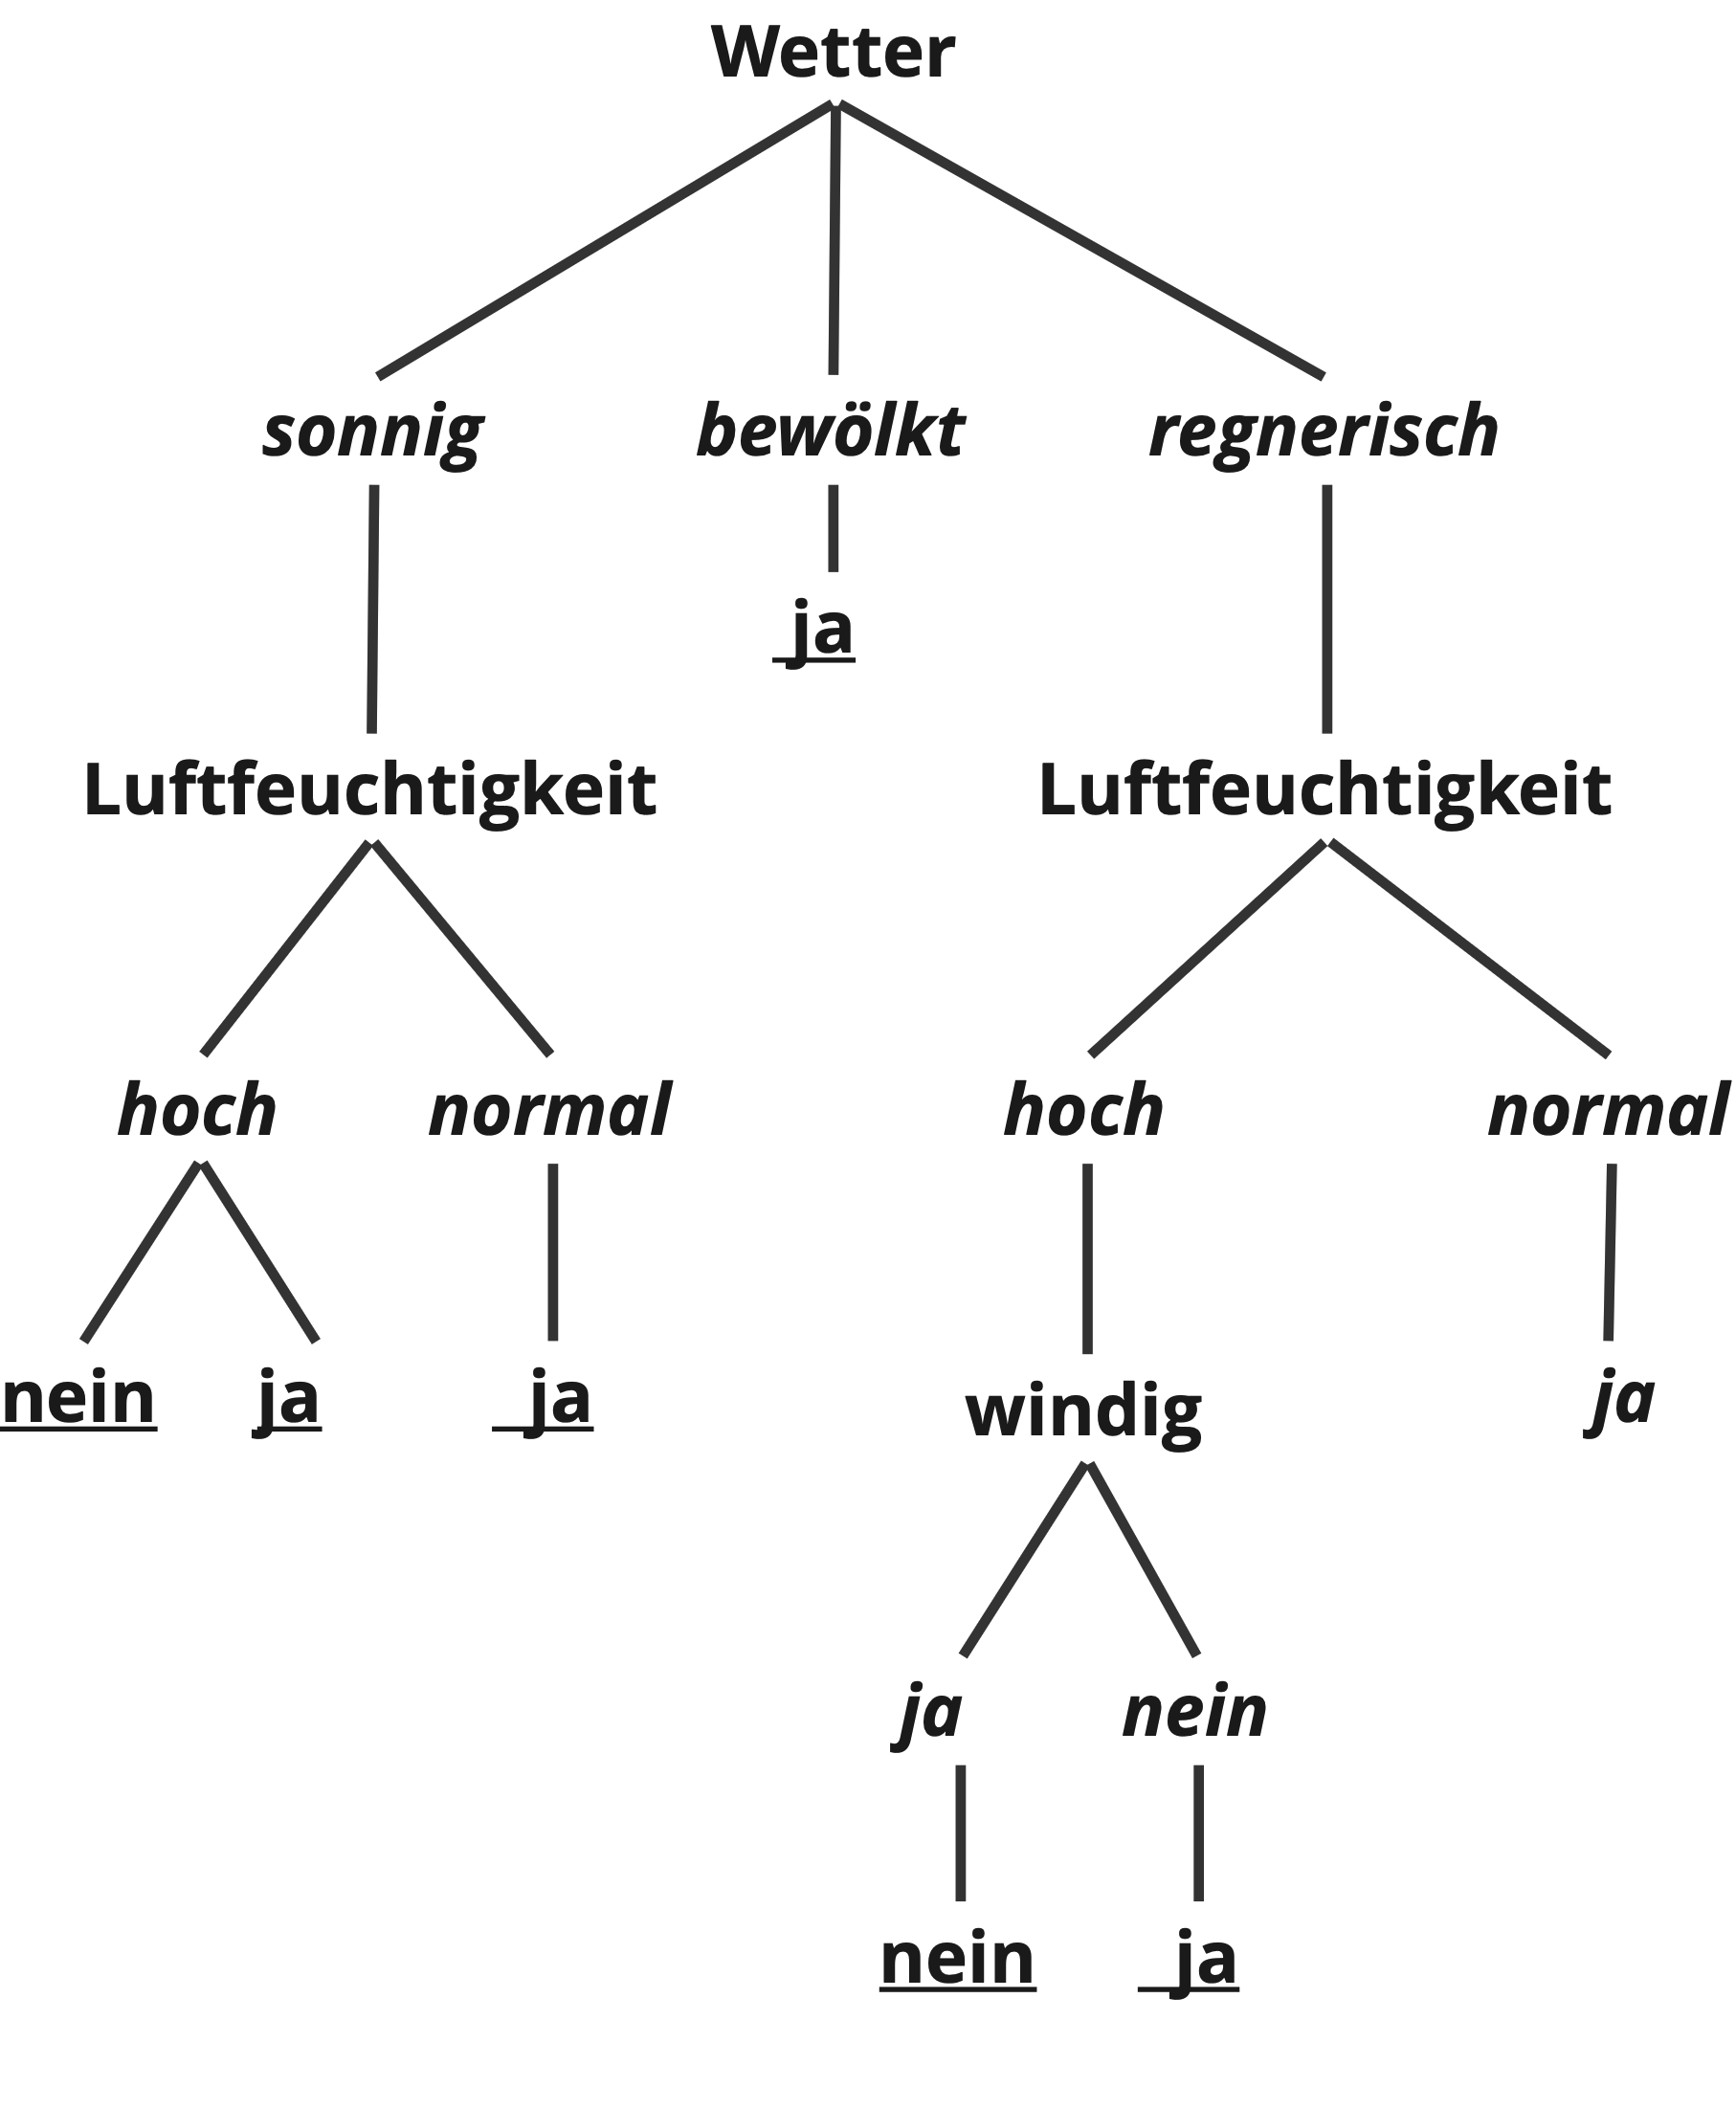
\includegraphics[width=\textwidth]{../Bilder/DT_ex.png}
        \caption{Beispielbild des resultierenden Decision Trees}
        \label{fig:example}
    \end{subfigure}
    \caption{Beispielhafte Darstellung Desicion Tree}
\end{figure}

Abbildung 2 stellt dies simplifiziert und beispielhaft da. Weiterhin wird der ID3-Algortihmus, welcher zur Errechnung des Information-Gains durch Entropie
benutzt wird offen gelassen und es wird auf die Quelle für diesen Abschnitt, ein grundlegendes Paper von J. Ross Quinlan, verwiesen. \cite{Quinlan1986}

Das Random-Forest Verfahren nutzt also diese Decision Trees und wendet weitere Techniken an, um deren schwächen zu negieren, diese lauten unter anderem wie folgt:

\begin{itemize}
    \item \textbf{Bootstrapping}: Aus dem ursprünglichen Datensatz werden durch Ziehen mit Zurücklegen mehrere neue Datensätze (Bootstrap-Samples) erstellt. Jeder dieser neuen Datensätze dient als Trainingsdatensatz für einen der Entscheidungsbäume.
    
    \item \textbf{Random Feature Selection}: Bei der Aufspaltung eines Knotens in jedem Entscheidungsbaum wird nicht der gesamte Satz von Features betrachtet, sondern nur eine zufällige Auswahl davon. Dies erhöht die Diversität der Bäume und verhindert, dass einzelne dominante Features alle Bäume gleich beeinflussen.
    
    \item \textbf{Training}: Jeder Entscheidungsbaum wird auf seinem jeweiligen Bootstrap-Sample und der zufälligen Auswahl von Features trainiert.
    
    \item \textbf{Aggregation}: Nachdem alle Entscheidungsbäume trainiert wurden, werden ihre Vorhersagen kombiniert. Bei Klassifikationsaufgaben wird in der Regel die Mehrheitsabstimmung verwendet, während bei Regressionsaufgaben der Durchschnitt der Vorhersagen genommen wird.
\end{itemize}

Dadurch erlangt das Verfahren einige Vorteile gegenüber der einzelnen Decision Tree Variante, wie der Resisitenz gegen Overfitting, einer niedrigeren Anfälligkeit für Ausreißer und einer meist
höheren Präzision als anderen herkömmlichen Klassifikatoren.

\subsection{Fallstudie RF}

Neben Siirtola et al. \cite{Siirtola2019} erzeugt \ac{RF} auch im Paper von Prerna et al. \cite{Prerna2021} die besten Ergebnisse. Es wird in diesem Abschnitt einmal Beispielsweise auf die Methodik dieses Papers eingegangen.

Verwandet wurde abermals der WESAD-Datensatz \cite{Schmidt2018WESAD}. Aus diesem wurden nur Sensordaten des RespiBAN für den weitern Verlauf verwendet, ergo unter anderem 
\ac{EKG}-Signale. 



\subsection{Unsupervised}

Ein im Vergleich relativ unerforschter Bereich ist die Anwendung von Unsupervised-Learning zur Klassifizierung von Stress, welches aber vorallem im Bezug auf Alltags-Wearables ausdrücklich attraktiv wirkt.

Kurz zusammengefasst stellen Unsupervised-Learning-Algortihmen eine Gruppe der Algorithmen des maschinellen Lernens ad, bei der ohne gelabelte Daten gearbeitet wird, 
um versteckte Muster oder Strukturen in den Eingabedaten zu entdecken, indem sie Ähnlichkeiten oder Unterschiede zwischen den Datenpunkten identifizieren und diese in Cluster, Assoziationen oder Hauptkomponenten 
einteilen.

Wie Iqbal et al. im für diesen Abschnitt benutzten Paper \cite{Iqbal2022} bereits schrieb, ist die geringe Verfügbarkeit von hochwertigen gelabelten Datensätzen eine sehr große Herausforderung
für die Entwicklung der Klassifizierungmodelle. Dies spiegelt sich auch darin wieder, dass man immer auf die gleichen verwerndeten Datensätze stößt. Weiterhin ist die Methodik der Erfassung der Labels, sei es durch Formulare im Nachgang oder durch beispielsweise \ac{TSST}
ein immernoch recht unentschlossener Punkt, da man immer auf Abweichungen in der Methodik der bereits verfügbaren Datensätze stösst.

Der Gedankengang keine gelabelten Daten zu benötigen, sondern stattdessen auf Unsupervised-Learning zu setzen ist also aufgrund dieses Punkt bereits einer näheren Untersuchung wert. Auf den Bezug zu Alltags-Wearables wird in Sektion 
7 ausdrücklicher eingegangen.

Diesen Vorteilen muss man allerdings einem eventuellen Performance-Verlust gegenüber klassischen Supervised-Learning Modellen 
entgegenstellen, was durch Iqbal et al. untersucht wurde.

Dieser zog zwei bereits erwähnte öffentlich verfügbare Datensätze heran (SWELL-KW \& Stress Recognition in Automobile Drivers) welche beide mehrere physiologische Marker beinhalten und gelabelt wurden.
Es wurden für je Kategorie Unsupervised-/Supervised-Learning sieben Algortihmen trainiert und evaluiert, je mit Angabe der Hyperparameter. Es wurde jeweils auf Herzrate und Atmung einzeln und in Kombination trainiert.

Bei der Feature auswahl ist anzumängeln, dass keine Begründung für die Wahl von nur einens beziehungsweise zweier Features angegeben wurde. Weitergehend ist auch der Prozess des Feature-Engineerings nicht
nachvollziehbar, es wurde nur erwähnt, dass die Daten von Ausreißern bereinigt wurden, jedoch nicht ob die Rohen \ac{EKG} Signale oder rausgerechnete Features verwendet wurden.

Das Resultat der Auswertung zeigte aber auf, das Unsupervised-Learning Algorithmen durchaus im Schnitt der Accuracy schlechter performten, dies aber nur marginal und durchaus auch Algortihmen dieser Kategorie
besser performen konnten als einiger des Supervised-Learning.

Das Ergbeniss stützt die mögliche Relevanz solcher Algorithmen für die Stress-Klassifizierung, weshalb in \cite{Iqbal2022} wie auch hier aufgefordert wird, mehr in diese Richtung zu forschen. Dies wird ich auch in der nächsten Sektion widerspiegeln.


\section{Proposal}
Betrachtet man die bisher identifizierten Challenges wie etwa die Sorge um Sensorungenauigkeiten bei Bewegung, die schwere Generalisierbarkeit von solchen Modellen, 
Abstinenz von hochqualitativen, balancierten Datensätzen und bisher keinem Modell auf rein physiologischen Markern jenseits der 90\% Accuracy stellt sich die Frage 
in welche Richtung man die Forschung fokussieren sollte, um diese zu mitigieren. Während der Literaturrechere kamen einige bisher unerschlossene Zweige, sowie bereits vorgeschlagen, vielversprechende
abweichende Ansätze auf. 

Wie bereits in Sektion 3.1.3 erwähnt, existieren Ansätze wie in Mozos et al. zur supplementären Analyse anderer Sensorik, hier soziometrische. Ein Alltags-Wearable bietet grundlegend auch die 
Möglichkeit solch andere Merkmale zu erfassen um eventuell die Accuracy von Modellen durch weitere aussagekräftige Features zu erhöhen. Ein interessanter Ansatz, welcher zwar noch nicht mit der bisher in Apple Watches verbauten 
Sensorik realisiert werden kann, aber, wie folgender im Februar 2024 veröffentlichter Patentantrag Apples \cite{Kim2024} in Aussicht stellt, ist die Messung der Cortisolkonzentration im Schweiß wie in Singh et al. \cite{Singh2023} dargestellt.

Das von Apple eingereichte Patent stellt zwar nur einen Sensor zur Messung der Schweißmenge und -rate in Aussicht, dennoch stellt eine Forschung in Richtung von Singh et al. eine wichtige Abzweigung da.

Ernst et al. stellten die Ergebnisse ihrer evaluierten physiologischen Marker bereits einer Messung des Cortisollevels im Speichel gegenüber, wobei ein Anstieg auf das Maxima nach etwa 18 Minute nach der Stressinduktion erfolgte. \cite{Ernst2023} 
Singh et al. suggeriert mit der Aussage, man Messe durch die Veränderung der Cortisolkonzentration nicht nur die nachfolgenden sonder verursachenten Effekte im Gegensatz zur Messung von physiologischen Markern, dass man einen schneller reagierenden Marker untersuche. 
Dies ist schlüssig mit den bisherigen Darlegungen der modernen Stressinterpretation, wenn auch in Sektion 2.1 die Cortisolausschüttung der \ac{HPA-Achse} bereits als 'langsamer' betitelt wurde, was die 18 Minuten von Ernst et al. stützt, aber eine Beobachtung der direkt induzierten Veränderung einem Laien dennoch sinnig vorkommt.

Kurzgefasst wurde ein neuartiges Wearable-Patch entworfen, welches sehr präzise die Cortisolkonzentration im Schweiß messen kann. Mit Verweiß auf \cite{Singh2023} zur Veranschauligung der konkreten Funktionsweise, weißt dies jedoch auch einige Challanges auf, 
wie der Notwendigkeit diese Sensoren nach einer gewissen Periode mithilfe einer Lösung auszuspülen um sie zu reaktivieren.

Zieht man noch den Schmerzpunkt des mangels an gelabelten Daten, sowie die von Siirtola et al. benutzten personalisierten Modelle, wird folgender Forschungsansatz vorgeschlagen:

Die Evaluierung eines Multisensorik-Wearable Systems, welches mithilfe der kontinuierlichen Messung von Herzfrequenz-Features sowie der Cortisolkonzentration im Schweiß durch Unsupervised-Learning Algortihmen personalisierte Modelle pro Probant erstellt.

Dieser Ansatz weißt einige Schwierigkeiten auf, stellt aber eine vielversprechende Alternative zu bisherigen Ansätzen da, welche sich ausschließlich auf physiologische Marker konzentrieren.
Dem vorher gehend benötigt es einiges an Forschung im Bereich des Unsupervised-Learnings zur Erstellung von Stressklassifizierungs-Modellen, sowie der Verbesserung der kontinuierlichen Cortisolkonzentrazionsmessung. Weiterhin ist unklar, ob Features aus diesen beiden Senoriksystemem supplementär oder konträr auf ein Klassifizierungsmodell wirken würden.

\section{Fazit}

Diese Arbeit hat den aktuellen Stand der Forschung zur Klassifizierung von Stresszuständen anhand von physiologischen Daten, die durch Wearables erfasst werden, untersucht. Stress ist in der modernen Gesellschaft ein allgegenwärtiges Problem, das durch verschiedene Faktoren verstärkt wird und erhebliche Auswirkungen auf die psychische und physische Gesundheit haben kann. Die traditionelle Forschung von Walter B. Cannon und Hans Selye bildet die Grundlage für unser Verständnis der physiologischen Stressreaktionen, während moderne Interpretationen von Wissenschaftlern wie David S. Goldstein diese Konzepte weiterentwickelt haben.

Die Analyse der technologischen Grundlagen von Wearables, insbesondere der Apple Watch, hat gezeigt, dass diese Geräte in der Lage sind, wichtige physiologische Marker wie die Herzfrequenz und die Herzratenvariabilität zu erfassen, die als Indikatoren für Stress dienen können. Die Validierung dieser Daten durch den WESAD-Datensatz hat gezeigt, dass es möglich ist, signifikante Unterschiede zwischen stressigen und stressfreien Zuständen zu erkennen.

In der Untersuchung der Methoden des maschinellen Lernens zur Klassifizierung von Stress wurde festgestellt, dass Random-Forest-Algorithmen besonders effektiv sind, da sie eine hohe Genauigkeit und Robustheit gegenüber Überanpassung bieten. Gleichzeitig wurde auf die potenziellen Vorteile unsupervised learning Algorithmen hingewiesen, insbesondere angesichts der Herausforderungen bei der Beschaffung gelabelter Datensätze.

Ein innovativer Ansatz, der in dieser Arbeit vorgeschlagen wird, ist die Kombination von kontinuierlichen Messungen der Herzfrequenz-Features und der Cortisolkonzentration im Schweiß mithilfe eines multisensorischen Wearable-Systems. Dies könnte die Genauigkeit der Stressklassifizierung weiter verbessern und bietet eine vielversprechende Richtung für zukünftige Forschung.

Zusammenfassend lässt sich sagen, dass die Nutzung von Wearables zur Erkennung und Überwachung von Stresszuständen ein vielversprechendes Feld ist, das durch die Weiterentwicklung von Sensortechnologien und Algorithmen des maschinellen Lernens erheblich profitieren kann. Die vorgeschlagenen Ansätze und Erkenntnisse dieser Arbeit könnten dazu beitragen, effektivere und individuell angepasste Lösungen zur Stressbewältigung zu entwickeln.
    
    
